%{{{
\documentclass{beamer}
\usetheme{ensam}
\usepackage{pgfplots}
\usepackage{amsmath}
\usepackage{subcaption}
\usepackage{multicol}
\usepackage{acronym}
\usepackage{tikz}
\usetikzlibrary{calc}
\usepackage{amsmath}
\usepackage {algorithmic}
\usepackage{algorithm}
\usepackage{eqparbox}
\usepackage[font=scriptsize]{caption}
\usetikzlibrary{bayesnet,positioning,calc}
\tikzstyle{obs} = [latent,fill=lightBlue]
\tikzstyle{default}=[draw=sexyRed,thick,rounded corners,text width=0.5in,font=\scriptsize,align=center]
\usepgfplotslibrary{colorbrewer}
\definecolor{ForestGreen}{RGB}{34,139,34}
\newcommand{\comment}[1]{\textcolor{ForestGreen}{#1}}
%algorithmic comment
\renewcommand\algorithmiccomment[1]{%
  \hfill\comment{\#\scriptsize\eqparbox{COMMENT}{#1}}%
}
\renewcommand{\algorithmicrequire}{\textbf{Input:}}
\renewcommand{\algorithmicensure}{\textbf{Output:}}
\title{Denombrement}
\author{\underline{A.Belcaid}}
\institute{\small ENSA-Safi} 

%tikz bayesian theme
\usetikzlibrary{bayesnet,positioning,calc}
\tikzstyle{obs} = [latent,fill=lightBlue]
\tikzstyle{default}=[draw=sexyRed,thick,rounded corners,text width=0.5in,font=\scriptsize,align=center]
\DeclareMathOperator{\argmin}{argmin}

\pgfplotsset{every tick label/.append style={font=\tiny}}




\begin{document}
\maketitle

\begin{frame}
\tableofcontents
\end{frame}
\section{Motivation}
\begin{frame}[t]
  \frametitle{Motivation}
  
  \begin{block}{Motivation}
    \scriptsize
    Un Entraineur de basketball doit choisir une équipe entre \textbf{30
    joueurs}. Son équipe se constitue de \textbf{5 joueurs} principaux et
    \textbf{7 remplacants}.\\[4pt] 
    \alert{\textbf{Quel est le nombre d'équipes qu'il peut choisir?}} 
  \end{block}
  \pause
\begin{itemize}
    \item Application principe simple de Dénombrement.\\[4pt]
    \item Applications:
      \pause
      \begin{multicols}{2}
       \begin{itemize}
       \item Permutations
        \item Combinaisons.
        \item Partitions
        \item Nombre de sous ensembles
        \item Probabilité binomiale.
      \end{itemize}
        
      \end{multicols}
  \end{itemize}

\end{frame}

\section{Principe de Denombrement}
\begin{frame}[t]
  \frametitle{Principe de Denombrement}
  \begin{columns}
    \begin{column}{0.5\textwidth}
     \begin{itemize}
       \item<1->   4 chemises.
       \item<1->   3 cravates.
        \item<1->  2 vestes.
     \end{itemize} 

     \begin{block}{Question}
       \scriptsize
       Quel est le nombre possible d'atours?
     \end{block}
     \begin{itemize}
       \item<2-> $r$ stages.
       \item<3-> $n_i$ choix par stage $i$.
     \end{itemize}
     \only<4->{
     \begin{block}{Calcul}
      \scriptsize 
       Le nombre de choix est :
       $$
       n_1 \times n_2 \ldots n_r
       $$
     \end{block}
   }
    \end{column}
    \begin{column}{0.5\textwidth}
     \only<2->{
         \centering
         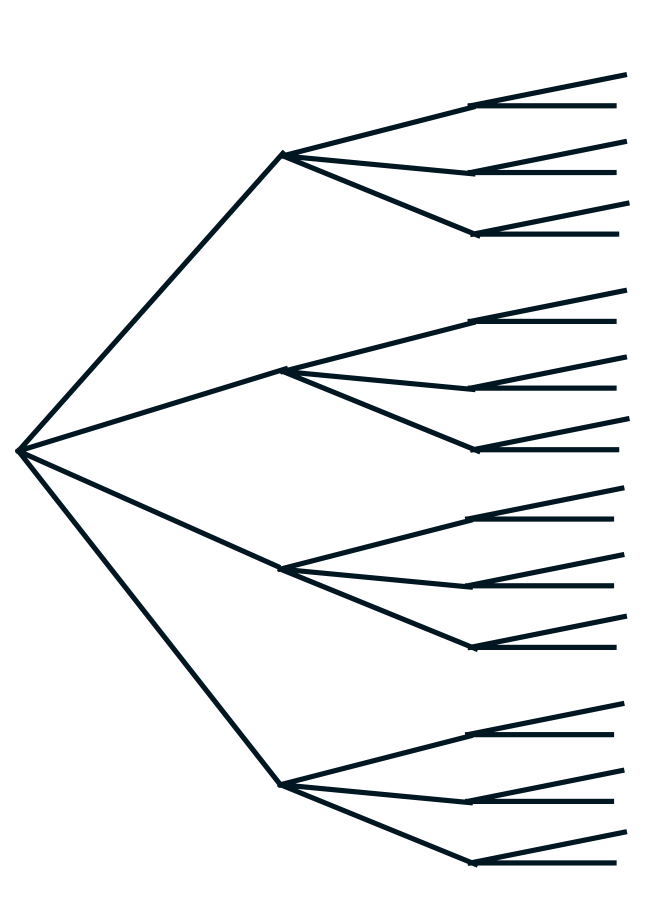
\includegraphics[width=0.8\textwidth]{./tree_example1.png}
     }
    \end{column}
  \end{columns}
\end{frame}

\begin{frame}[t]
  \frametitle{Exemples}
  \begin{itemize}
    \small
    \item  Le nombre de licences de voitures avec deux lettres et 3 chiffres?
    \item<2-> 
      \begin{equation*}
        26\times 26 \times 10 \times 10 \times 10
      \end{equation*}
      \begin{itemize}
        \item<3-> Et si les lettres et les chiffres ne peuvent pas être répétées?
        \item<4->
          \begin{equation*}
            26 \times 25 \times 10 \times 9 \times 8
          \end{equation*}
      \end{itemize}
    \item<5-> \alert{\textbf{Permutations}}: On suppose qu'on a ensemble de $n$
      éléments. Par combien de méthodes on peut les \textbf{Ordonner}?
    \item<6->
      \begin{equation*}
        n! = n\times(n-1)\times \ldots 1
      \end{equation*}

    \item<7-> \alert{Nombre de sous ensembles} de $\{1,\ldots, n\}$.
      \begin{equation*}
        2\times 2 \times \ldots \times 2 = 2^n 
      \end{equation*}
  \end{itemize}
\end{frame}
  
\begin{frame}[t]
\frametitle{Exemple}
 \begin{block}{Exemple}
   \scriptsize
\begin{itemize}
  \item On lance un de a six faces.\\[4pt]
    Calculer la probabilité que tous les des donnent un valeur
    \alert{\textbf{différente}}.\\[4pt]
\end{itemize}
 \end{block} 
 \pause
 \begin{itemize}
   \item 
     $$
     card(\Omega) = 6^6
     $$
 \end{itemize}

 
 \pause

 \begin{itemize}
   \item
     $$
     card(A) = 6\times 5 \times\ldots 1 = 6!
     $$
     \pause

     $$
     \mathbf{P}(A) = \dfrac{6!}{6^6}
     $$
 \end{itemize}
\end{frame}

\section{Combinaisons}
\begin{frame}[t]
  \frametitle{Combinaisons}
 \begin{block}{Définition}
   \small
   Le nombre \alert{$\binom{n}{k}$} représente le nombre de sous-ensembles contenant $k$
   éléments d'un ensemble avec $n$ éléments.
 \end{block} 
\pause
 \begin{itemize}
   \scriptsize
   \item  On peut trouver cette formule on choisissant tout d'abord un séquence
     ordonnée de $k$ éléments.
     $$
     \begin{array}{|c|c|c|c|c|c|}
       \hline
       n & (n-1) &  & &  & (n-k + 1)\\
       \hline
     \end{array}
     $$
     \pause
  \begin{equation*}
    n(n-1)\ldots (n-k + 1) = \dfrac{n!}{(n-k)!}
  \end{equation*}
  \vspace*{1cm}
\item Maintenant si on veut éliminer l'ordre puisqu'il compte pas, on obtient
  alors:
  \begin{equation}
    \binom{n}{k} = \dfrac{n!}{(n-k)!k!}
  \end{equation}
 \end{itemize}
\end{frame}

\begin{frame}[<+->]
  \frametitle{Combinaisons}
  
  \begin{itemize}
  \small
    \item 
    \begin{equation*}
    \binom{n}{k} = \dfrac{n!}{(n-k)!k!}
    \end{equation*}
    \\[8pt]
    \item 

    \begin{equation*}
    \binom{n}{n} = \dfrac{n!}{(0)!n!} = 1
    \end{equation*}

    \item 

    \begin{equation*}
    \binom{n}{0} = \dfrac{n!}{(n)!0!} = 1
    \end{equation*}
    \\[8pt]
    \item 
    \begin{equation*}
    \sum_0^n \binom{n}{k} = 
    \end{equation*}
  \end{itemize}
\end{frame}
\begin{frame}[t]
  \frametitle{Exercise}
 \begin{block}{Enonce}
 \scriptsize
 On dispose de $n$ fonctionnaires et on veut choisir une \textbf{comite} avec un
 chair (chef). La comité doit consister de $k\geq 1$ personnes.\\[4pt]
 \end{block} 
 \begin{itemize}
 \scriptsize
   \item<1-> Calculer alors combien de comité on peut choisir avec $k$ personnes
   \pause
   $$
   k\binom{n}{k}
   $$
   \item<3-> Maintenant on cherche a calculer la somme de tous les choix
   possibles pour $k$
   $$
   c = \sum_{k=1}^n k\binom{n}{k}
   $$
   \pause
   Calculer la valeur de $c$. Un petit indice, vous devez trouver une expression
   de la forme 
   $$
   c = (\alpha + n^\beta)2^{\gamma n  + \delta}
   $$
 \end{itemize}
\end{frame}
\begin{frame}[<+->]
  \frametitle{Probabilites Binomiale}
  
  \begin{itemize}
  \small
    \item \textbf{Coefficient binome} $\binom{n}{k}\longrightarrow$  :
    \alert{\textbf{probabilite de binome}}.\\[8pt]
    \begin{itemize}
      \item $n\geq 1$ lance \alert{\textbf{independant}}  d'une pièce de
      monnaie: $\alert{\mathbf{P}(H) = p}$.
      \item Quelle est la probabilité d'obtenir \textbf{\structure{k Heads}}.
      $$
      \mathbf{P}(\text{\scriptsize k heads}) = 
      $$
\item $P(HTTHHH) = $\\[8pt]
\item $P(\text{\scriptsize sequence paticuliere})$ \\[8pt]
\item $P(\text{\scriptsize sequence particuliere avec k H})$\\[8pt]
\item $P(\text{\scriptsize sequence avec k H})$
    \end{itemize}
  \end{itemize}
\end{frame}

\begin{frame}[t]
  \frametitle{Exercise}
  \begin{block}{Exercice}
On as lance une pièce de monnaie   $\mathbf{10}$ fois et on sait qu'on
as obtenu $\mathbf{3}$ H.\\[4pt]

Quelle est la urobiline que les \alert{\textbf{deux premiers}}  lances ont donne
$H$?
\end{block}
\end{frame}


\section{Partitions}
\begin{frame}[t]
  \frametitle{Partitions}
 \begin{itemize}
 \small
   \item<1-> On dispose de $\alert{n} \geq 1$ éléments distincts.
   \item<2->  On possède $\alert{r}$ personnes.
   \begin{block}{Question}
    Comment distribuer $n_i$ éléments pour chaque personne $i$. 
   \end{block}
   \begin{itemize}
     \item On suppose que les $n_1, n_2,\ldots, n_r$ sont des entiers naturels.
     \item Tel que $n_1 + n_2 + \ldots + n_r = n$
   \end{itemize}
   \pause
 \end{itemize} 

   \begin{block}{Nombre de partition}
     \small
     Le nombre de partitions est:
     \begin{equation}
     \dfrac{n!}{n_1!n_2!\ldots n_r!}\quad {\alert{\text{Coefficient multinomial}}}
     \end{equation}
   \end{block}
\end{frame}
\begin{frame}[<+->]
  \frametitle{Exercise}
  \begin{block}{Énonce}
  \scriptsize
    
    On dispose de 9 objets qu'on veut distribuer a trois personnes.
    \begin{itemize}
    \scriptsize
      \item Akram doit avoir $\mathbf{2}$
    \item Brahim doit avoir $\mathbf{3}$.
    \item Chaimae doit avoir $\mathbf{4}$.
    \end{itemize}
  \end{block}
 \begin{enumerate}
   \item Calculer par combien de façon on peut distribuer des objets.\\[1cm]
   \item Une autre façon d'obtenir ce résultat est tout d'abord de choisir
   \textbf{deux} objets pour Akram. 
   \begin{itemize}
     \item Calculer le nombre de scénario pour réaliser ceci.\\[4pt]
   \end{itemize}
   \item Maintenant, il nous reste $\mathbf{7}$ objets qu'on doit distribuer a
   Brahim et Chaimae.
   \begin{itemize}
     \item Calculer par combien de façon on peut réaliser ceci.\\[4pt]
     \item Comparer maintenant les deux resultats.
   \end{itemize}
 \end{enumerate} 
\end{frame}

\begin{frame}[t]
  \frametitle{Jeu de carte}
  
  \begin{block}{Jeu de carte}
  \small
  On dispose dans jeu de carte contenant \alert{$\mathbf{52}$}. Ce jeu de carte
  est distribue a \textbf{quatre} joueurs.\\[8pt]

  \alert{Calculer la probabilite que chaque joueur obtient un As}?
    
  \end{block}
  \pause
    \begin{itemize}
      \scriptsize
      \item  Nombre de cas possibles
      $$
      card(\Omega) = \dfrac{52!}{4\cdot (13!)}
      $$
      \pause
    \item Calculer le nombre de cas pour obtenir le résultat: 
      \begin{itemize}
        \scriptsize
        \item Distribuer les As.
          \pause
          $$
          4\cdot 3 \cdot 2 \cdot 1
          $$
          \pause
        \item Distribuer les 48 cartes restantes.
          \pause
          $$
          \dfrac{48}{4\cdot(12!)}
          $$
      \end{itemize}
    \end{itemize}
\end{frame}
\end{document}
